\documentclass[UTF8]{ctexart}
\usepackage{enumerate}
\usepackage{amssymb}
\usepackage{graphicx}
\usepackage{subfigure}
\usepackage{amsmath}
\usepackage{geometry}
 \usepackage{indentfirst} 
 \usepackage{listings}
 \usepackage{xcolor}


\lstset{
    backgroundcolor=\color{red!50!green!50!blue!50},%代码块背景色为浅灰色
    rulesepcolor= \color{gray}, %代码块边框颜色
    breaklines=true,  %代码过长则换行
    numbers=left, %行号在左侧显示
    numberstyle= \small,%行号字体
    keywordstyle= \color{blue},%关键字颜色
    commentstyle=\color{gray}, %注释颜色
	frame=shadowbox%用方框框住代码块
}
\begin{document}
	\title{\textbf{《数据库》课程实践报告}\\[1ex]
	\begin{large}
		Efficient Subgraph Matching
	\end{large}}
	\author{姓名:蒋慧\,\,学号:51194501050\,\,专业:软件工程}
	\maketitle

\section{引言}
\par{
在本次项目实践中,我们组选取了子图匹配问题,该问题提取了大数据图G中查询图q的所有子图同构嵌入。
子图匹配的现有算法遵循Ullmann的回溯方法;也就是说,通过遵循查询顶点的匹配顺序,
将查询顶点迭代映射到数据顶点。已经表明,查询顶点的匹配顺序对于子图匹配算法的效率非常
重要。近年来,已提出了许多高级技术,例如增强连接性和在查询或数据图中合并相似的顶点,
以提供有效的匹配顺序,目的是减少中间结果,特别是由冗余笛卡尔积引起的中间结果。在本文中
,我们第一次解决了来自“异类”顶点的笛卡尔积的无结果结果的问题。我们通过推迟基于查询结
构的笛卡尔乘积来提出一个新框架,以最大程度地减少冗余笛卡尔乘积。我们的第二个贡献是提出了
一种新的基于路径的辅助数据结构,其大小为 $O(|E(G)| × |V(q)|)$,以生成匹配顺序并进
行子图匹配,这非常重要减小现有基于路径的辅助数据结构的指数大小 $ O(|V(G)|^{|V(q)|−1})$,
其中$V(G)$和$E(G)$是数据的顶点和边集分别是图$G$和$V(q)$是查询$q$的顶点集。对实图
 和合成图的大量实证研究表明,我们的技术比最先进的算法高3个数量级。
}
\par{SPath是一种新的图形索引技术,可以有效解决大型网络上的图形查询问题。
它为每个查询顶点维护一个邻域签名-一种在顶点附近存储分解的最短路径信息的结构。
SPath彻底改变了图形查询处理方式,从一次顶点到一次路径,这比传统的图匹配方法更具成本效益。
}
\section{相关工作}
\par{
	CPI就是为了生成一个有效的匹配顺序,以迭代方式将一个顶点从查询图映射到数据图,以最大程度地减少中间结果的总数。
	 QuickSI提出了基于不频繁标签优先策略生成匹配顺序的方法。 SPath提出基于不频繁路径优先策略生成匹配顺序,
	 以解决仅考虑QuickSI中的顶点和边的局限性。 $Turbo_{ISO}$技术提出了精确枚举所有路径的方法,以克服SPath的局限性,
	 后者可能会通过估算公式高估连接基数。
}
\section{问题描述}
\par{在此次实验中我们遇到的问题主要有一下几个方面:
}
\begin{enumerate}[(1)]
	\item 异构顶点的冗余笛卡尔积。
	\item $Turbo_{ISO}$ 中基于路径的数据结构的指数大小。

\end{enumerate}
\section{方案及实现}
\par{
根据我们组内分工,我主要负责进行自底向上的细化方法,用于进一步细化查询顶点的候选对象。
和neo4j可视化部分,算法首先将查询图q按照深度分层,对于每一层分别处理,处理过程分为两个部分:向前处理以及向后处理。
向前处理维护两个集合N与UN,分别保存已经访问的顶点与这一层还未访问的顶点,同时维护集合C,保存这个节点所能匹配的候选结点。
由于向前遍历时没有考虑到当前层还未访问结点的连接情况,所以每当一层遍历完以后,会执行向后处理,将后续结点的信息考虑进去,
更新每个结点的候选集合C。由于自顶向下的构造只能根据父结点的信息进行构造,所以需要自底向上的细化过程,将孩子结点的信息考虑进去,
自底向上的细化过程如图2所示。算法从最低层开始,逐层向上更新候选集合C,判断上层结点的候选集是否和下层结点的候选集有至少一条边相连,
若找不到这样的一条边,则把该结点从候选集中删除。我将自底向上的算法进行了实现,具体的代码实现见附录1。我们自下而上从u3开始,因为u3这一层没有别的结点,不需要处理,然后看u2,因为u2和u3有边,所以u2.C必须和u3.C的任意一个节点有边连接,所以去掉v8,接下来也是同理,时间关系我就不讲了。最后我们就得到了一个较为小的一个CPI,如图2。

\begin{figure}[h]
	\centering
	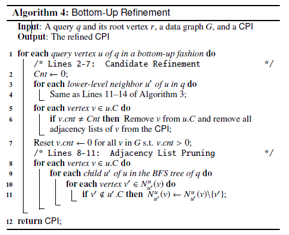
\includegraphics[width=7cm,height=7cm]{/Users/jiangqianxi/Desktop/github/Quantum-Computation-and-Quantum-Information/数据库论文/WechatIMG6.png}
	\caption{自底向上的算法}
	\end{figure}

}
\par{
	下面是构造CPI的例子,主要是修剪无效的候选人,计算有效的匹配顺序。
	\begin{figure}[htbp]
		\centering
		\subfigure[CPI]{
		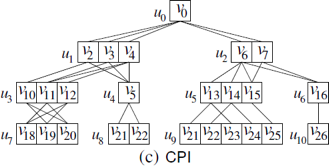
\includegraphics[width=5.5cm]{/Users/jiangqianxi/Desktop/github/Quantum-Computation-and-Quantum-Information/数据库论文/WechatIMG14.png}
		%\caption{fig1}
		}
		\quad
		\subfigure[数据图]{
		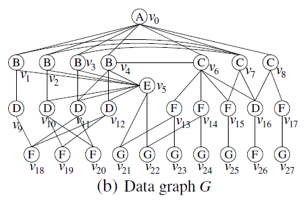
\includegraphics[width=5.5cm]{/Users/jiangqianxi/Desktop/github/Quantum-Computation-and-Quantum-Information/数据库论文/WechatIMG13.png}
		}
		\quad
		\subfigure[查询图]{
		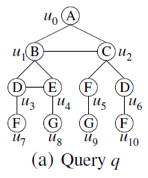
\includegraphics[width=5.5cm]{/Users/jiangqianxi/Desktop/github/Quantum-Computation-and-Quantum-Information/数据库论文/WechatIMG12.png}
		}
		\quad
		\subfigure[Core-Forest-Leaf]{
		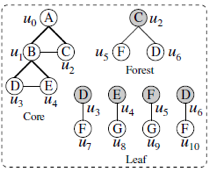
\includegraphics[width=5.5cm]{/Users/jiangqianxi/Desktop/github/Quantum-Computation-and-Quantum-Information/数据库论文/WechatIMG15.png}
		}
		\caption{ 自底向上构造过程}
		\end{figure}
	
}

\par{
我负责的第二部分就是将结果在 $Neo4j$ 上可视化, $Neo4j$ 是一个嵌入式,基于磁盘的,支持完整事务的Java持久化引擎,
它在图(网络)中而不是表中存储数据。 $Neo4j$ 提供了大规模可扩展性,在一台机器上可以处理数十亿节点/关系/属性的图,
可以扩展到多台机器并行运行。相对于关系数据库来说,图数据库善于处理大量复杂、互连接、低结构化的数据,这些数据变化迅速,
需要频繁的查询——在关系数据库中,这些查询会导致大量的表连接,因此会产生性能上的问题。 $Neo4j$ 重点解决了拥有大量连接的
传统RDBMS在查询时出现的性能衰退问题。通过围绕图进行数据建模, $Neo4j$ 会以相同的速度遍历节点与边,其遍历速度与构成
图的数据量没有任何关系。我们将节点和边的关系丢到 $Neo4j$ 中,然后他就会直观的帮我们进行构造出这些图,测试代码见附录。
}
\par{
	$ Neo4j$ 主要操作方法如下:
	\begin{enumerate}[(1)]
		\item 实体(Entity)\\
		是指节点(Node)和关系(Relationship);\\
		每个实体都有一个唯一的ID;\\
		每个实体都有零个,一个或多个属性,一个实体的属性键是唯一的;\\
		每个节点都有零个,一个或多个标签,属于一个或多个分组;\\
		每个关系都只有一个类型,用于连接两个节点;\\
		
		
		\item 	路径(Path)\\
		是指由起始节点和终止节点之间的实体(节点和关系)构成的有序组合;\\
		\item 标记(Token)\\
		是非空的字符串,用于标识标签(Lable),关系类型(Relationship Type),或属性键(Property Key);\\
		标签:用于标记节点的分组,多个节点可以有相同的标签,一个节点可以有多个Lable,Lable用于对节点进行分组;\\
		关系类型:用于标记关系的类型,多个关系可以有相同的关系类型;\\
		属性键:用于唯一标识一个属性;\\
		\item 属性(Property)\\
		是一个键值对(Key/Value Pair),每个节点或关系可以有一个或多个属性;属性值可以是标量类型,或这标量类型的列表(数组);
		
	\end{enumerate}
	
}
\section{课程总结}
\par{
	通过数据这门课,通过老师的讲解,我学到了数据库的一些原理上的知识,但是后续如果有需要还需要自己深入学习,
	老师讲授结束后,每位同学都会选择一篇论文阅读分享,这篇论文算是我真正意义上读的第一篇顶会论文,通过这篇论文的
	阅读,我感受到科研的魅力,大概了解自己接下来的研究生生涯是怎样的,读了这篇论文,稍微扩展了我的知识面,
	偷窥了图数据库的冰山一角,感觉好难啊,然后和优秀的同学组队做了一个project,感受到团队合作的魅力,
	我们做的是一篇论文的实现,通过这次实践加深了对这篇论文算法的理解,但是由于课程时间问题,同学们讲论文的时间很不够,
	就不能很好的展现一篇顶会的魅力,由于时间来不及了,有的同学就是放ppt,这样感觉违背了老师的初衷。
}
\section{附录}
\par{
	附录1:
	\begin{figure}[h]
		\centering
		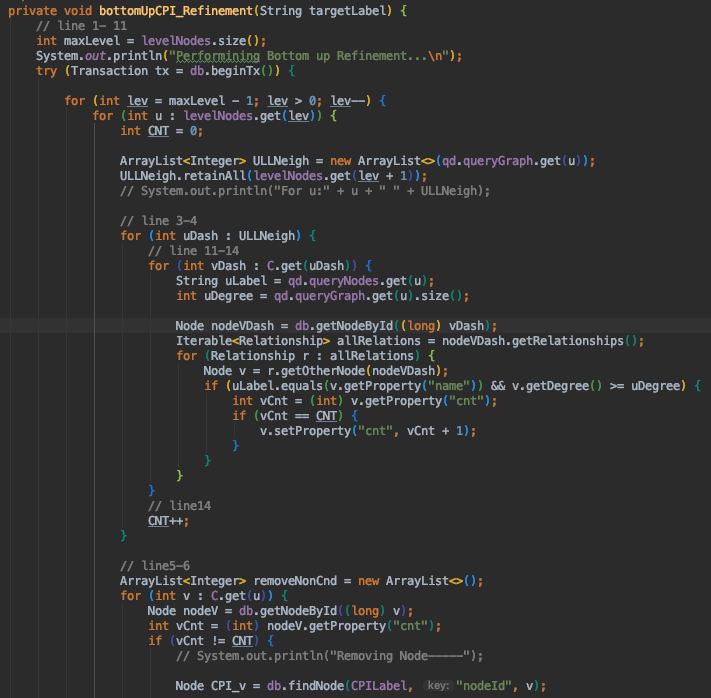
\includegraphics[width=14cm,height=14cm]{/Users/jiangqianxi/Desktop/github/Quantum-Computation-and-Quantum-Information/数据库论文/WechatIMG9.png}
		\caption{自底向上的算法代码1}
	\end{figure}
	\begin{figure}[h]
			\centering
			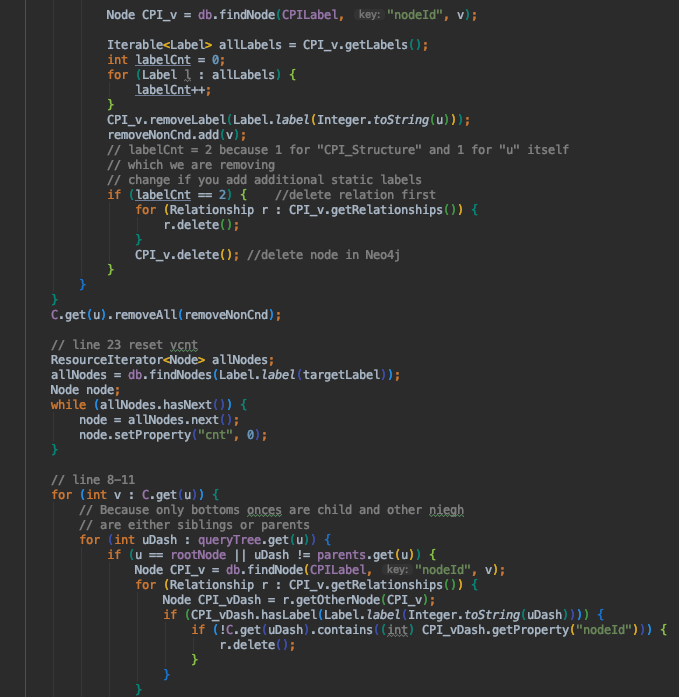
\includegraphics[width=14cm,height=14cm]{/Users/jiangqianxi/Desktop/github/Quantum-Computation-and-Quantum-Information/数据库论文/WechatIMG10.png}
			\caption{自底向上的算法代码2}
	\end{figure}
\begin{figure}[h]
	\centering
	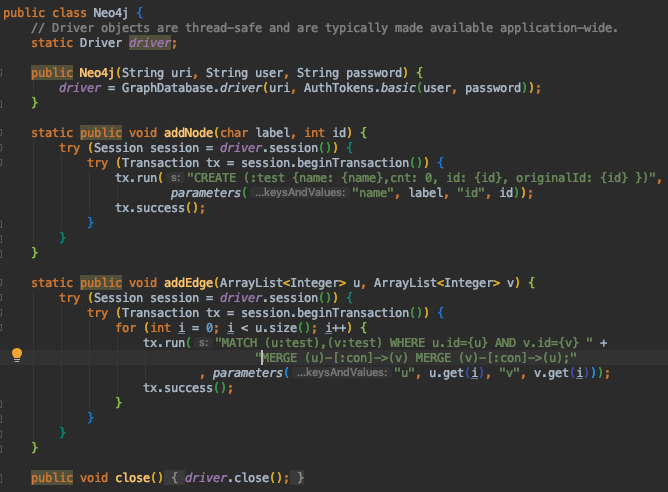
\includegraphics[width=14cm,height=14cm]{/Users/jiangqianxi/Desktop/github/Quantum-Computation-and-Quantum-Information/数据库论文/WechatIMG11.png}
	\caption{$Neo4j$ 测试代码}
\end{figure}
}

% ---- Bibliography ----
\bibliographystyle{unsrt}
\bibliography{cite}

\end{document}